\section{Expérience B3} 
  \subsection{Objectif}
    Reproduction et approfondissement des résultats de la première expérience 1 dans l'article 
    \cite{Cleeremans_2007}. 

  
  
    Comprendre de quelles manières peuvent émerger des représentations et méta-représentations dans 
    un réseau de neurone connexionniste, en particulier sur des perceptrons multicouches.
  
  
  \subsection{Architecture}
    \paragraph{Description}
      Un premier réseau de perceptron multicouche apprend à discrétiser des chiffres représentés
      par 20 neurones d'entrées. Il est composé d'une couche cachée de 5 neurones.
      
      Un second réseau de perceptron multicouche apprend à dupliquer toutes les couches du premier
      réseau en n'ayant que sa couche cachée en entrée.
      
      L'apprentissage du second réseau, n'affecte pas les poids entre la couche d'entrée et la 
      couche cachée du premier réseau.

    \paragraph{Schéma}
      \begin{center}
	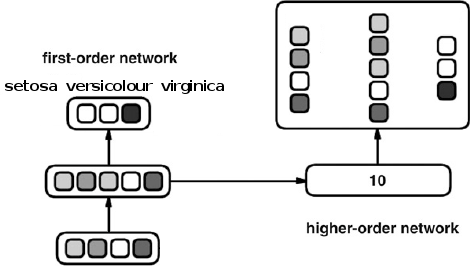
\includegraphics[width=220px]{data/expA4/schema.png}
      \end{center}
      
    \paragraph{Paramètres}
      \begin{center}
	\begin{tabular}{lr}
	  \begin{minipage}{230px}
	    \begin{itemize}
	      \item momentum : 0.9 sur les 2 réseau
	      \item taux d'apprentissage : 0.1 sur les 2 réseau
	      \item 10 chiffres différents présentés
	      \item apprentissage 10 (formes) x 1000 (époques)
	      \item utilisation de biais
	    \end{itemize}
	  \end{minipage}
	  &
	  \begin{minipage}{230px}
	    \begin{itemize}
	      \item poids initialisés sur [-0.25 ; 0.25]
	      \item taux d'apprentissage constant
	      \item entrées valent 0 ou 1
	      \item sigmoïde à température 1
	    \end{itemize}
	  \end{minipage}
	\end{tabular}
      \end{center}

  
  \newpage
  \subsection{Résultats}
    \paragraph{Principaux}
      Analyse des performances
      \begin{center}
	\begin{tabular}{lr}
	  \hspace*{-1cm}
	  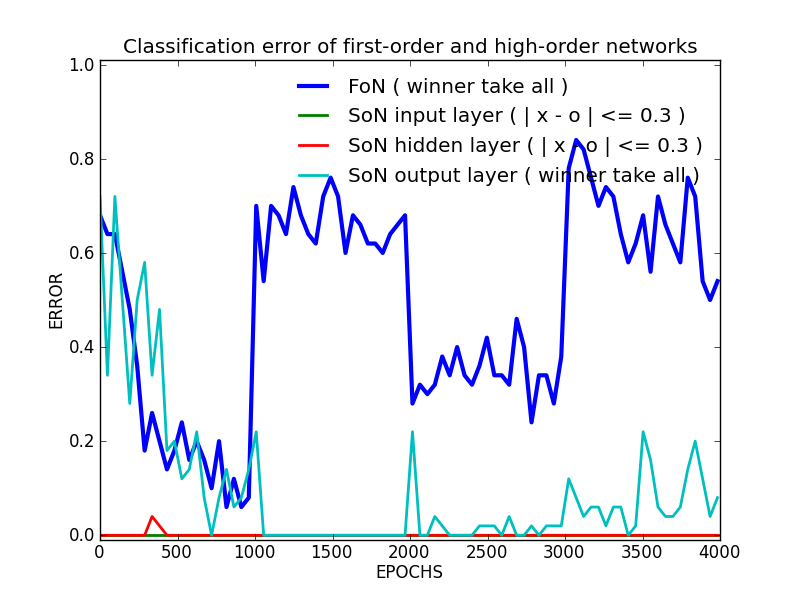
\includegraphics[width=250px]{data/expB3/err.png}
	  &
	  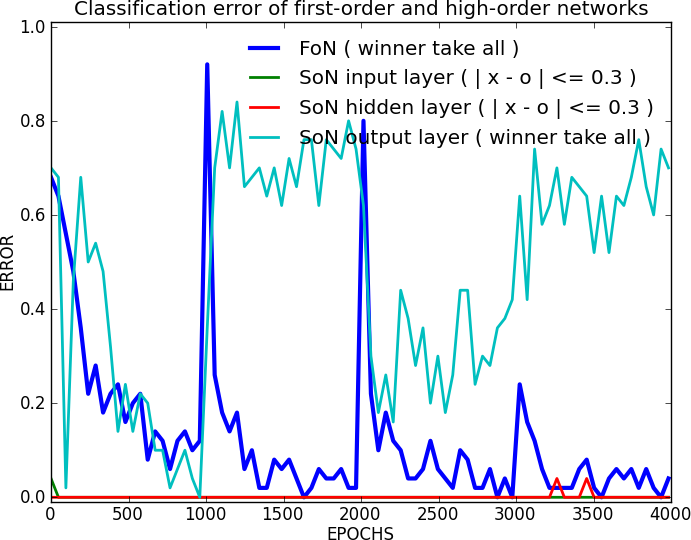
\includegraphics[width=250px]{data/expB3/err_block.png} 
	\end{tabular}
      \end{center}
      \subparagraph{Notes}
	\begin{itemize}
	  \item les courbes SoN layer représentent les erreurs (du second réseaux) des couches du premier à reproduire 
	  \item la courbe RMS verte (SoN) est la somme des 3 courbes SoN layer
	\end{itemize}
      \subparagraph{Conclusion}
	\begin{itemize}
	  \item la couche cachée et la couche de sortie ne posent aucun problèmes d'apprentissage
	  \item les performances du second réseau dépendent principalement de sa capacité à reproduire les entrées
	  \item le second réseau apprend plus rapidement que le premier
	\end{itemize}
    \paragraph{Secondaires}
      RMS
      \begin{center}
	\begin{tabular}{lr}
	  \hspace*{-1cm}
	  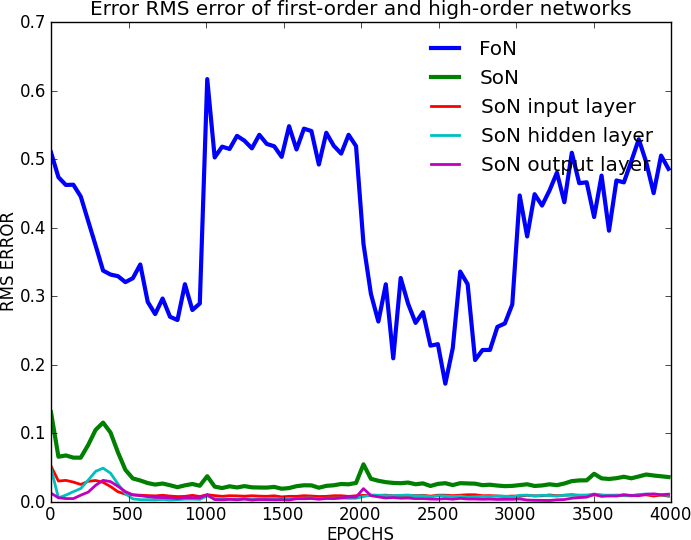
\includegraphics[width=250px]{data/expB3/rms.png}
	  &
	  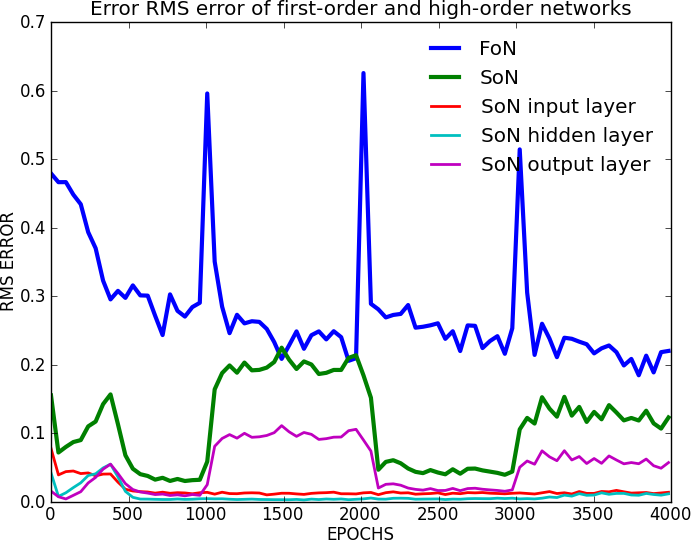
\includegraphics[width=250px]{data/expB3/rms_block.png} 
	\end{tabular}
      \end{center} 
      \subparagraph{Notes}
	\begin{itemize}
	  \item une couleur équivaut à un chiffre présenté
	  \item une valeur discretisée correspond à un certain encodage de la couche cachée (cf Algorithmes)
	\end{itemize}
      \subparagraph{Conclusion}
	Les neurones se stabilisent très rapidement (autour de la 50\up{ième} époque en moyenne), 
	le tout permettant au second réseau d'avoir des entrées très peu variables, favorisant
	son apprentissage.
    \paragraph{Secondaires}
      Représentations au travers des poids du premier réseau
      \begin{center}
	Couche cachée \\
	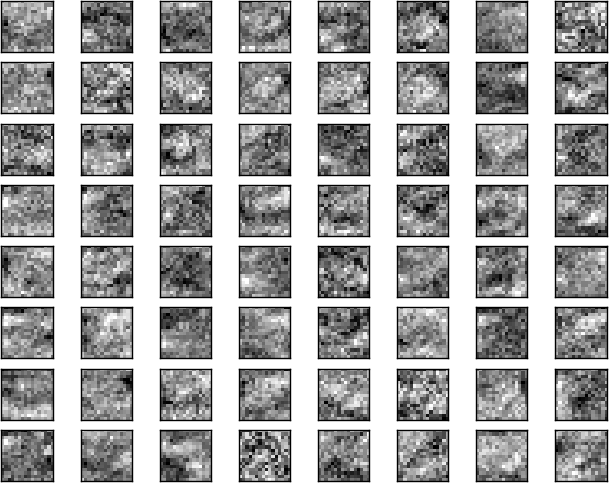
\includegraphics[width=250px]{data/expA3/representation_hidden.png}
      \end{center}
      \begin{center}
	Couche de sortie \\
	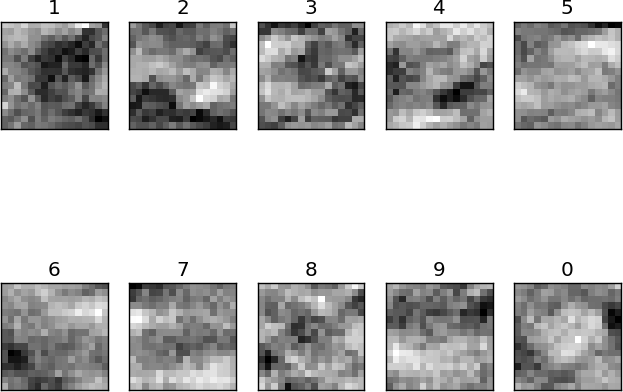
\includegraphics[width=250px]{data/expA3/representation.png}
      \end{center} 
      \subparagraph{Notes}
	\begin{itemize}
	  \item plus une case est noire, plus sa présence est importante pour le chiffre en question
	  \item plus une case est blanche, plus son absence est importante
	\end{itemize}
      \subparagraph{Conclusion}
	Il est assez difficile d'y distinquer les chiffres, mais cela semble suffisant pour le réseau
	qui a un taux de reconnaissance de 100\%.

      \subparagraph{Conclusion}
	Le peu d'entrées permet l'apprentissage par-coeur de chaque forme.
	


  \subsection{Conclusion}
  
  

  \newpage 
  \subsection{Formules}
    \paragraph{RMS} \label{rms}
  Pour une époque $e$ :
  \begin{center}
    \begin{large}
    $ rms_{e} = \sqrt{ \frac{1}{n} \sum \limits_{i=1}^{n} 
    ( o_{i,e} - d_{i} )^2 } $
    \end{large}
  $ with \left\lbrace \begin{array}{lll} n : number\ of\ neurons\ on\ the\ output\ 
  layer\\o_{i,e} : value\ obtained\ for\ the\ i^{th}\ neuron\ at\ the\ e^{th}\ epoch\\d_{i} : 
  value\ desired \ for\ the\ i^{th}\ neuron\end{array} \right.$
  \end{center}
    \paragraph{Discrétisation} \label{discretize}
      Pour la couche cachée $hiddenNeuron$ de $n$ neurones, un neurone
      pouvant être encodé par $number\_cutting$ valeurs différentes :
      \begin{center}
	$\sum \limits_{i=0}^{n} number\_cutting^{i} \times cutting(hiddenNeuron[i]) $
      \end{center}
      \subparagraph{Exemple}
	$400 \gets [0 ; 0,25 ]\ [0 ; 0,25 ]\  [0,25 ; 0,5 ]\  [0,5 ; 0,75 ]\  [0,25 ; 0,5 ]$ \\
	\hspace*{2.70cm}
	$400 \gets 0\times4^0 +   0\times4^1  +   1\times4^2   +  2\times4^3   +   1 \times4^4$
    \paragraph{Descente de gradient} \cite{Touzet_1992} \\
  Construction de l'erreur : 
    \begin{center}
      $y_{i} = f'(a_i) \times ( d_i - x_i ) \ si\ i\ neurone\ de\ sortie $ \\
      $y_{i} = f'(a_i) \times \sum \limits_{k} ( w_{ki} \times y_k )\ si\ i\ neurone\ cache $
    \end{center}
  Mise à jour des poids :
    \begin{center}
      $w_{ij}(t+1) = w_{ij}(t) + learning\_rate \times y_{i} \times x_j + momentum \times 
      (w_{ij}(t) - w_{ij}(t-1) )$
    \end{center}
  Variables : 
    \begin{center}
      $\left\lbrace \begin{array}{lll} 
	f : fonction\ sigmoide \\
	x_i : valeur\ du\ neurone\ i\\
	d_i : valeur\ desire pour\ le\ neurone\ i\\
	a_i : somme\ pondere\ des\ poids\ du\ neurone\ i
      \end{array} \right.$
    \end{center}

\bibliographystyle{../pre-rapport/apalike}
\bibliography{../pre-rapport/biblio}
